\documentclass{article}

\usepackage[english]{babel} %Forces American English hyphenation patters
\usepackage[utf8x]{inputenc} % Unicode
\usepackage{amsmath, amssymb, amsthm} %AMS Math Packages
\usepackage{textcomp, siunitx, gensymb, wasysym} %Symbol Packages, Textcomp removes certain errors
\usepackage{multicol, geometry, fancyhdr} %Page Layout Packages 
\usepackage{graphicx, wrapfig, subcaption} %Figure Packges
\usepackage{hyperref}
\usepackage{algorithm}
\usepackage[noend]{algpseudocode}

\renewcommand{\l}{\left}
\renewcommand{\r}{\right}

\graphicspath{ {./images/} }
\geometry{margin = 1in}
\setlength{\parindent}{0pt}

\pagestyle{fancyplain}
\headheight 1cm
\lhead{Michael Dymek \\ \today}
\chead{\textbf{\Large The n-Body Problem}}
\rhead{Dr. Larson \\ Computational Physics}
\headsep .5cm

\begin{document}
\section*{Problem}
For this project, I will investigate a gravitational system involving $n$ bodies. For two bodies, there exists a general analytic solution for the subsequent motion of the given bodies. This cannot be said about any more than that though, which is what leads to the $n$ body problem. When given the initial position and velocity of $n$ bodies with known masses, find the subsequent motion of the $n$ bodies.
	
\section*{Theory}
Our ultimate goal here is to develop a method for finding the motion of $n$ bodies under each others gravitational influence. We know from Newton's second law that $\ddot{x} = \frac{F}{m}$, and that the gravitational force on each body $u$ will be
\[ F_{G,u} = \sum_{u \neq v} \frac{G m_u m_v}{r_{u,v}^2}\hat{r}_{u,v}. \]
For each dimension, we will need to take the portion of the force that is in that dimension, which results in the following equation for the acceleration of the $u^{\text{th}}$ body in the $s$ direction:
\[ a_{u,s} = \sum_{u \neq v} \frac{G m_v \Delta s_{u,v}}{r_{u,v}^3}. \]
From there, we can use the Euler-Cromer method to find the changes in velocity and position of each body. I will be performing this simulation in two dimensions, but this can generalize to any number of dimensions quite easily. For each of the bodies, we will follow the following algorithm to calculate their subsequent position.
\begin{algorithm}
	\caption{Euler-Cromer Gravitational Motion}
	\label{alg:Gravitational_Motion}
	\begin{algorithmic}
		\State For each time step $i$, calculate $v$ and $x$ at time step $i+1$.
			\begin{itemize}
				\item[$\blacktriangleright$] Calculate the distance $r$ between each of the objects.
				\begin{itemize}
					\item[$\blacklozenge$] $r_{u,v} = \sqrt{\l(x_u - x_v\r)^2 + \l(y_u - y_v\r)^2}$.
				\end{itemize}
				\item[$\blacktriangleright$] Calculate the accelerations of each body in the $x$ and $y$ directions.
				\begin{itemize}
					\item[$\blacklozenge$] $a_{u,x} = \sum_{u \neq v} \frac{Gm_v \Delta x_{u,v}}{r_{u,v}^3}$.
					\item[$\blacklozenge$] $a_{u,x} = \sum_{u \neq v} \frac{Gm_v \Delta y_{u,v}}{r_{u,v}^3}$.
				\end{itemize}
				\item[$\blacktriangleright$] Calculate the velocities of each body in the $x$ and $y$ directions.
				\begin{itemize}
					\item[$\blacklozenge$] $v_{x,i+1} = v_{x,i} + \l(a_x\r)\Delta t$
					\item[$\blacklozenge$] $v_{y,i+1} = v_{y,i} + \l(a_y\r)\Delta t$
				\end{itemize}
				\item[$\blacktriangleright$] Calculate the changes in the $x$ and $y$ positions for each body.
				\begin{itemize}
					\item[$\blacklozenge$] $x_{i+1} = x_{i} + \l(v_{x,i+1}\r)\Delta t$
					\item[$\blacklozenge$] $y_{i+1} = s_{i} + \l(v_{y,i+1}\r)\Delta t$
				\end{itemize}
				\item[$\blacktriangleright$] Iterate the time variable: $t_{i+1} = t_i + \Delta t$
				\item[$\blacktriangleright$] Repeat for the desired number of steps.
			\end{itemize}
	\end{algorithmic}
\end{algorithm}
\section*{Methods}
The main goal of my project here is to recreate analytic results that have been found by Chenciner and Montgomery \cite{Solution}. They found that there is an analytic periodic solution to the three body problem (a subset of the $n$ body problem) where the bodies move in a nice figure-eight pattern shown in Figure \ref{sfig:Figure_Eight_Solution}. \medskip

\begin{figure}[ht]
	\centering
	\begin{subfigure}{0.49\textwidth}
		\centering
		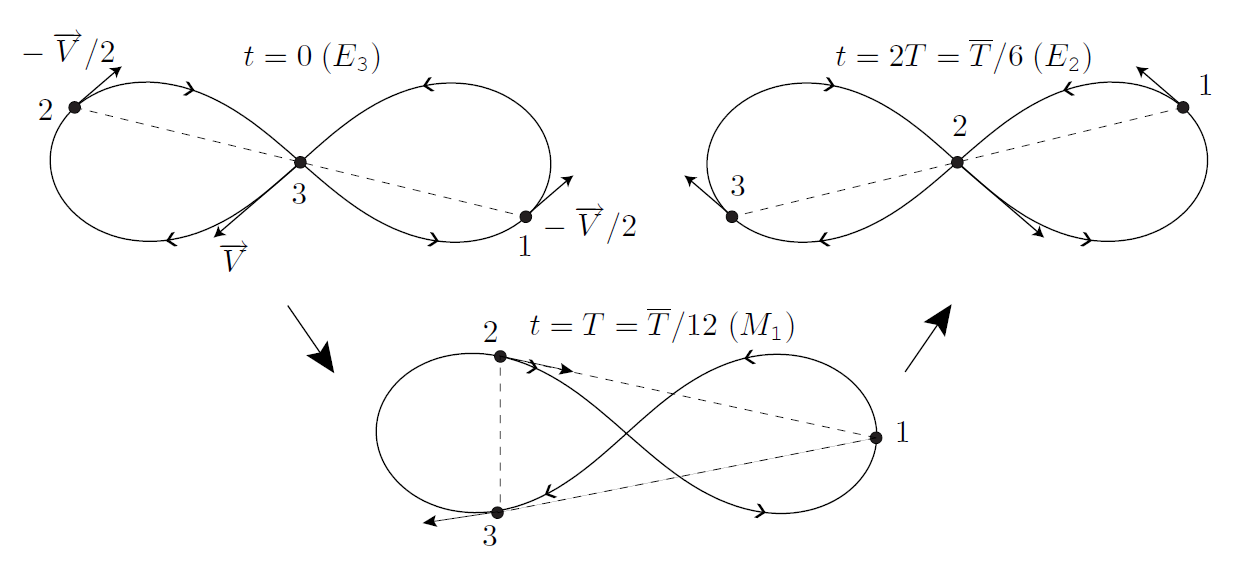
\includegraphics[width = \textwidth]{Figure_Eight_Solution.png}
		\caption{}
		\label{sfig:Figure_Eight_Solution}
	\end{subfigure}
	\begin{subfigure}{0.49\textwidth}
		\centering
		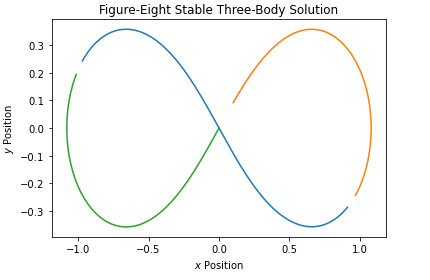
\includegraphics[width = \textwidth]{Figure_Eight_Solution_Simulation.png}
		\caption{}
		\label{sfig:Figure_Eight_Solution_Simulation}
	\end{subfigure}
	\caption{}
\end{figure}

For the simulation, I used initial conditions where $G = 1$, $r_1 = -r_2 = \l( 0.970 , -0.243 \r)$, $r_3 = (0,0)$, $v_3 = -2v_1 = -2v_2 = \l(-0.932, -0.865\r)$, and $m_1 = m_2 = m_3 = 1$. Running this simulation for $\SI{2}{\second}$, we find the result in Figure \ref{sfig:Figure_Eight_Solution_Simulation}. What we see is that the motion of the bodies definitely matches the analytic solution we were given. In this solution, the period of the motion is $T \approx 6.33$, which matches the result that we have, as each of the bodies does not quite complete a third of it's motion in the 2 second simulation. Running this simulation for longer, we can see whether or not the solution that we have is stable. \medskip

\begin{figure}[ht]
	\centering
	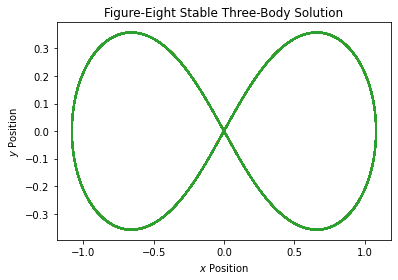
\includegraphics[width = 0.6\textwidth]{Figure_Eight_Solution_Long_Term.png}
	\caption{}
	\label{fig:Figure_Eight_Solution_Long_Term}
\end{figure}

In Figure \ref{fig:Figure_Eight_Solution_Long_Term}, we can see the path traced out by a single body over the course of $\SI{1000}{\second}$. This is a great result, as it helps to show that this is a stable orbit. This result is very interesting, as it implies that it is possible for this orbit to be found in real life. 

\section*{Future Work}
There are a lot of things that I would like to look into with this simulation. One things that would be really interesting is to look into the true average distances between each planet. A paper was released a few years ago that showed that Mercury is actually the closest planet to every other planet on average. I would love to use this simulation to see if I can duplicate those results.

\begin{thebibliography}{9}
\bibitem{Solution} 
Alain Chenciner and Richard Montgomery
\textit{A remarkable periodic solution of the three-body problem in the case of equal masses}. 
Annals of Mathematics, 152 (2000), 881-901.
\end{thebibliography}

\end{document}